\chapter{INTRODUCTION} \label{ch:intro}

\section{Motivation}
  Given the global rise in population, efficient and innovative resource utilization is increasingly important.
In particular, food and fuel are clearly in high demand.
Meanwhile, growing concern for the negative environmental impacts of petroleum-based fuel is generating a market for biofuel, especially corn-based ethanol.
However, corn-based ethanol has been heavily criticized for diverting land usage away from food production.
At the same time, a great deal of unutilized saltwater coastline is available for both food and fuel production through seaweed cultivation.
Specifically, the sugar kelp \textit{Saccharina Latissima} is known to be a viable source of food, both for direct human consumption and for fish cultivation, as well as for biofuel production.

%TODO: Nitrogen concerns, wastewater treatment.
Furthermore, nitrogen leakage into water bodies is a significant ecological danger, and is especially relevant near large conventional agriculture facilities due to run-off from nitrogen-based fertilizers, as well as near wastewater treatment plants.
As a specific example, there is a wastewater treatment plant in Boothbay Harbor, Maine which is facing increasingly demanding EPA regulations limiting the concentration of certain nutrients permissible to be released into the ocean via wastewater treatment outfalls.
In order to adhere to these stricter requirements using conventional nutrient remediation, a significant quantity of specialized equipment would be necessary, which is not currently present in the Boothbay Harbor plant.
Being surrounded on all sides by water and private property, the treatment plant lacks the necessary space for the additional equipment, and would therefore need to move their entire facility to a new location in order to conform to these new nutrient regulations.
As an alternative to conventional nutrient remediation techniques, the cultivation of the macroalgae \textit{Saccharina Latissima} (sugar kelp) near the outfall site has been proposed.
The purpose of such an undertaking would be twofold: to prevent eutrophication of the surrounding ecosystem by sequestering the nutrients in question, and to reduce the need for nutrient input, which is one of the largest costs in macroalgae cultivation. %TODO: Cite

Once grown, a variety of products can be derived from macroalgae, including biofuel, fish/cattle feed stock, and high value chemical materials such as alginate and agar.
Food for human consumption is also a common product of kelp aquaculture, though it may not be ideal for a wastewater treatment application.
Thus, there is an ongoing effort to investigate the feasibility, and optimal implementation of kelp farming in wastewater treatment operations. 

Industrial scale macroalgae cultivation has long existed in Eastern Asia due to the popularity of seaweed in Asian cuisine.
  More recently, kelp aquaculture has been developing in Scandinavia and in the Northeastern United States.
For example, the MACROSEA project is a four year international research collaboration funded by the Research Council of Norway targeting ``successful and predictable production of high quality biomass thereby making significant steps towards industrial macroalgae cultivation in Norway.'' %TODO: Cite this
The project includes both cultivators and scientists, working to develop a precise understanding of the full life cycle of kelp and its interaction with its environment.
A fundamental aspect of this endeavor is the development of mathematical models to describe the growth of kelp.
Work is underway at SINTEF, a private Norwegian research institution, to develop such models.
Ole Jacob Broch is a mathematician at SINTEF, a research organization in Trondheim, Norway, who has been working to model the growth of \textit{Saccharina Latissima} using SINMOD, a large-scale 3D hydrodynamical ocean model developed at SINTEF which generates data on water temperature, water velocity, light intensity, and phytoplankton concentrations among other valuable quantities \cite{wassmann_modelling_2006}.

One aspect of the model which has yet to be fully developed is the availability of light, considering factors such as absorption and scattering by the aquatic medium, as well as by the kelp itself.
In this thesis, we contribute to this effort by developing a first-principles model of the light field in a kelp farming environment.
As a first step, a model for the spatial distribution of kelp is developed.
Radiative transfer theory is then applied to determine the effects of the kelp and water on the availability of light throughout the medium.
We pursue a numerical finite difference solution to the Radiative Transfer Equation, and subsequently discuss asymptotic approximations which prove to be sufficiently accurate and less computationally intensive.
We also provide a detailed description of the numerical solution of this model, accompanied by source code for a FORTRAN implementation of the solution.
This model can be used independently, or in conjunction with a life cycle kelp model to determine the amount of light available for photosynthesis at a single time step.

\begin{figure}[h]
  \centering
  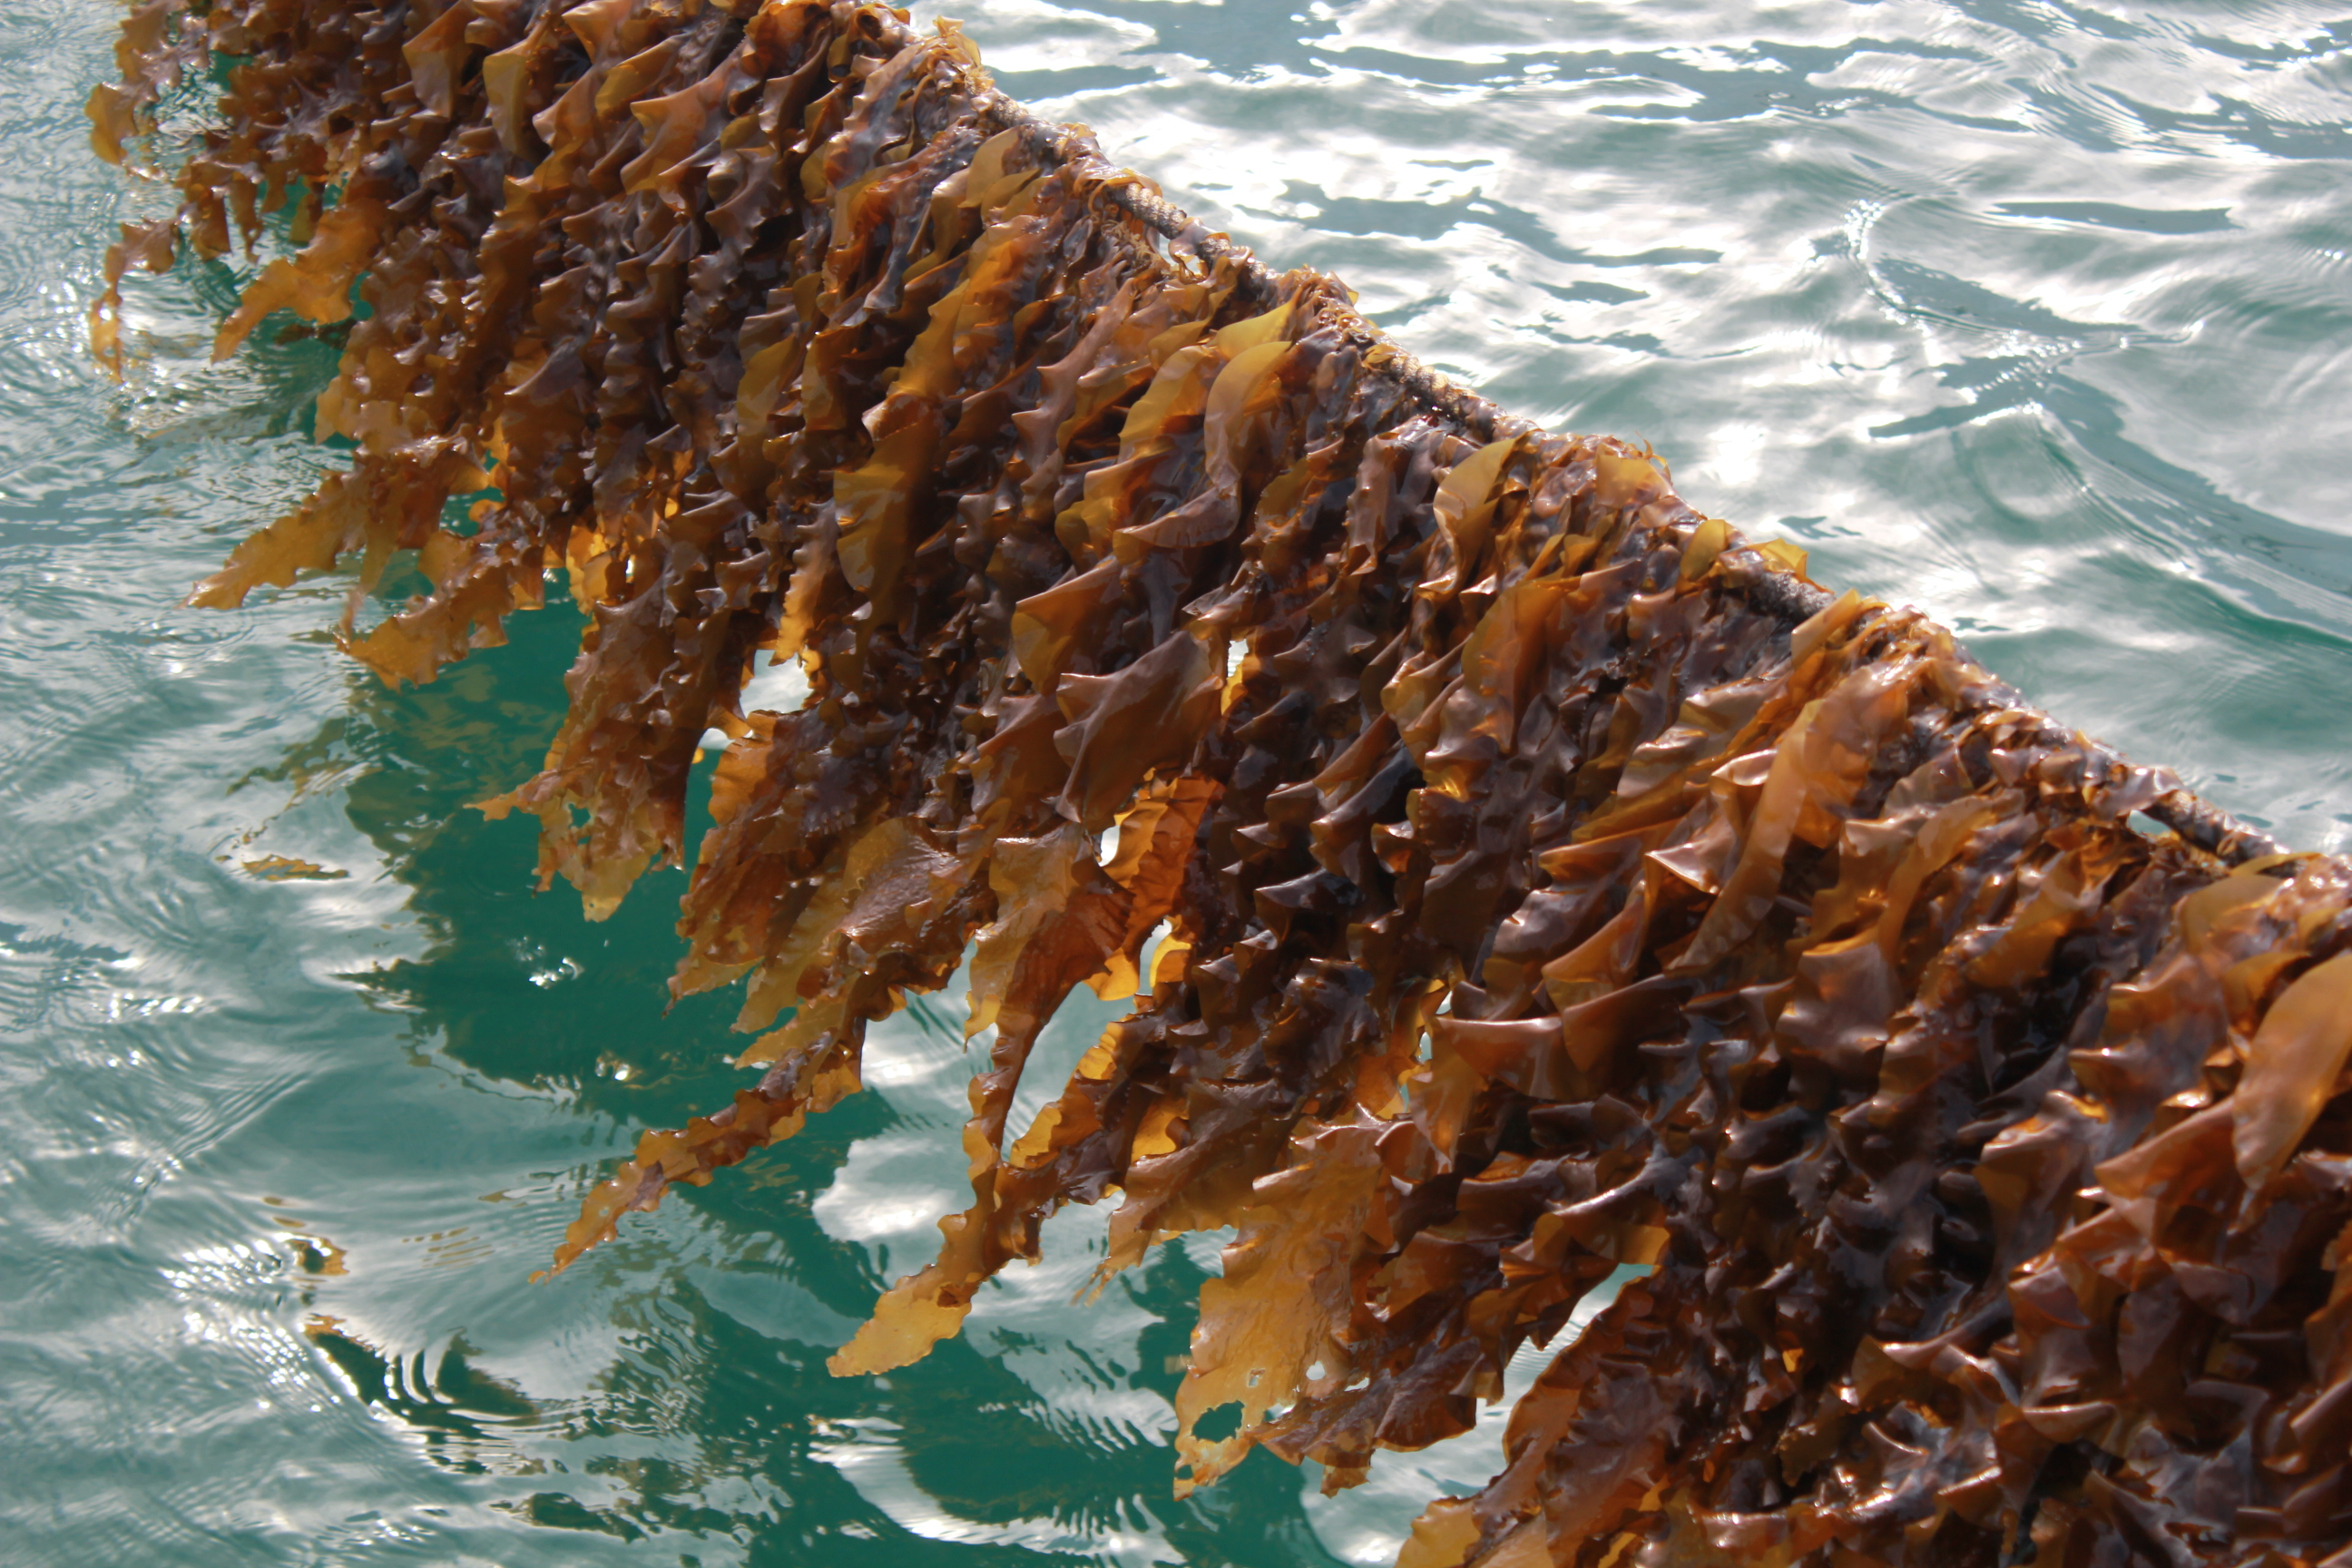
\includegraphics[width=\textwidth]{kelp_photo/kelp_photo1}
  \caption{\textit{Saccharina Latissima} being harvested}
  % https://blogs.qub.ac.uk/qubio/files/2016/04/H5-5.jpg
  %TODO: Cite properly or replace with photo from Shane
\end{figure}


\section{Background on Kelp Models}

Mathematical modeling of macroalgae growth is not a new topic, although it is a reemerging one.
Several authors in the second half of the twentieth century were interested in describing the growth and composition of the macroalgae \textit{Macrocystis pyrifera}, commonly known as ``giant kelp,'' which grows prolifically off the coast of southern California.
The first such mathematical model was developed by W.J. North for the Kelp Habitat Improvement Project at the California Institute of Technology in 1968 using seven variables.
By 1974, Nick Anderson greatly expanded on North's work, and created the first comprehensive model of kelp growth which he programmed using FORTRAN \cite{anderson_mathematical_1974}.
In his model, he accounts for solar radiation intensity as a function of time of year and time of day, and refraction on the surface of the water.
He uses a simple model for shading, simply specifying a single parameter which determines the percentage of light which is allowed to pass through the kelp canopy floating on the surface of the water.
He also accounts for attenuation due to turbidity using Beer's Law.
Using this data on the availability of light, he calculates the photosynthesis rates and the growth experienced by the kelp. \\[-0.75em]

Over a decade later in 1987, G.A.
Jackson expanded on Anderson's model for \textit{Macrocystis pyrifera}, with an emphasis on including more environmental parameters and a more complete description of the growth and decay of the kelp \cite{jackson_modelling_1987}. 
He takes into account respiration, frond decay, and most importantly for my work, sub-canopy light attenuation due to self-shading.
He simply adds a coefficient to the exponential decay of light as a function of depth to represent shading from kelp fronds.
He doesn't consider and radial nor angular dependence on shading. %TODO:  Check this. Was previously ambiguous.
Jackson also expands Anderson's definition of canopy shading, treating the canopy not as a single layer, but as 0, 1, or 2 discrete layers, each composed of individual fronds.
While this is a significant improvement over Anderson's light model, it is still rather simplistic. \\[-0.75em]

Both Anderson's and Jackson's model were carried out by numerically solving a system of differential equations over small time intervals.
In 1990, M.A. Burgman and V.A. Gerard developed a stochastic population model \cite{burgman_stage-structured_1990}.
This approach is quite different, and functions by dividing kelp plants into groups based on size and age, and generating random numbers to determine how the population distribution over these groups changes over time, based on measured rates of growth, death, decay, light availability, etc.
That same year, Nyman et. al. tested a similar model in New Zealand, as well as a Markov chain model, and compared the results with experimental data \cite{nyman_macrocystis_1990}. \\[-0.75em]

In 1996 and 1998 respectively, P. Duarte and J.G. Ferreira used the size-class approach to create a more general model of macroalgae growth, and Yoshimori et. al. created a differential equation model of \textit{Laminaria religiosa} with specific emphasis on temperature dependence of growth rate \cite{duarte_model_1997,yoshimori_mathematical_1998}.
These were the some of the first models of kelp growth that did not specifically relate to \textit{Macrocystis pyrifera} (``giant kelp''). 
Initially, there was a great deal of excitement about this species due to it's incredible size and growth rate, but difficulties in harvesting and negative environmental impacts have caused scientists to investigate other kelp species. \\[-0.75em]

\section{Background on Radiative Transfer}
In terms of optical quantities, our primary interest is in the radiance at each point from all directions, which affects the photosynthetic rate of the kelp, and therefore the total amount of biomass producible in a given area as well as the total nutrient remediation potential.
The equation governing the radiance throughout the system is known as the Radiative Transfer Equation (RTE), which has been largely unutilized in the fields of oceanography and aquaculture.
Meanwhile, it has been studied extensively in two fields: stellar astrophysics and computer graphics.
In its full form, radiance is a function of 3 spatial dimensions, 2 angular dimensions, and frequency, making for an incredibly complex problem.
In this work, frequency is ignored, only monochromatic radiation is considered.
The RTE states that along a given path, radiance is decreased by absorption and scattering out of the path, while it is increased by emission and scattering into the path.
In our situation, emission is negligible, owing only perhaps to some small luminescent phytoplankton or some such anomaly, and can therefore be safely ignored.

We use monochromatic radiative transfer in order to model the light field in an aqueous environment populated by vegetation.
The vegetation (kelp) is modeled by a spatial probability distribution, which we assume to be given.
The two quantities we seek to compute are \textit{radiance} and \textit{irradiance}.
Radiance is the intensity of light in at a particular point in a particular direction, while irradiance is the total light intensity at a point in space, integrated over all angles.
The Radiative Transfer Equation is an integro-partial differential equation for radiance, which has been used primarily in stellar astrophysics; it's application to marine biology is fairly recent \cite{mobley_radiative_2001}.

Understanding the growth rate and nutrient recovery by
kelp cultures has important marine biological implications. For example, recent
work by our research group at Clarkson University, the University of Maine, and
SINTEF Fisheries and Aquaculture is investigating kelp aquaculture as a means to
recover nutrients from wastewater effluent plumes in coastal environments into a
valuable biomass feedstock for many products. Current models for kelp growth
place little emphasis on the way in which nearby plants shade one another.
Self-shading may be a significant model feature, though, as light availability
may impact the growth and composition of the kelp biomass, and thus the mixture
of goods that may be derived.

\section{Overview of Thesis}
The remainder of this document is organized as follows.
In Chapter \ref{chap:kelp}, we develop a probabilistic model to describe the spatial distribution of kelp by assuming simple distributions for the lengths and orientations of fronds.
We begin Chapter \ref{chap:light} with a survey of fundamental radiometric quantities and optical properties of matter.
We use the spatial kelp distribution from Chapter \ref{chap:kelp} to determine optical properties of the combined water-kelp medium.
We then present the Radiative Transfer Equation, an integro-partial differential equation which describes the the light field as a function of position and angle.
An asymptotic expansion is explored for cases where absorption dominates scattering in the medium, such as in very clear water or high kelp density.
In Chapter \ref{chap:numerical}, details are given for the numerical solution of the equations from Chapters \ref{chap:kelp} and \ref{chap:light}.
Both the full finite difference solution and the asymptotic approximation are described.
Next, in Chapter \ref{chap:parameters}, we discuss the availability of necessary parameters in the literature.
For those which are not readily available, we give rough estimates and briefly describe experimental methods for their determination.
Then, in Chapter \ref{chap:model_analysis}, we investigate the necessary grid resolution for adequate accuracy in the full finite difference solution and compare to the asymptotic approximation for a few parameter sets.
Further, we determine the effect of varying a few key parameters on the light field predicted by the asymptotic approximation.
Afterwards, we use the light model developed here in a full lifecycle simulation of kelp growth and compare the light field and biomass production to those predicted by a simpler 1D exponential decay light model.
Finally, we conclude with Chapter \ref{chap:conclusion} by giving a brief summary of the model, discuss and its performance, and suggest improvements and avenues for future work.
